\documentclass[a4paper,11pt]{scrartcl}
\usepackage[utf8x]{inputenc}
\usepackage[catalan]{babel}
\usepackage{titlesec}
% A ses llengües llatines, el primer paràgraf ha d'anar tabulat
\usepackage{indentfirst}
\usepackage{amsmath}
\usepackage{float}
\usepackage{graphicx}
\usepackage{subfigure}
\usepackage{booktabs}
\usepackage{multirow}
\usepackage{hyperref}
\usepackage{url}
\usepackage{multirow}
\usepackage{minted} %wget http://minted.googlecode.com/hg/minted.sty

% aptitude install texlive-fonts-extra
\usepackage{newcent} %font mes wapa

\graphicspath{{diagrames/}}

% Estil de seccions
\titleformat{\section}{\large\sectfont}{\thesection}{1em}{}
\titleformat{\subsection}{\bfseries\sectfont}{\thesubsection}{1em}{}
% Estil numeracio subseccions http://help-csli.stanford.edu/tex/latex-sections.shtml#number
%\def\thesubsection{\alph{subsection})}

\title{Robòtica: \\ Raiden Project}
\author{ Bartomeu Miró Mateu \thanks{bartomeumiro a gmail punt com} \\
	 Lluis Cortès Rullan \thanks{lluisbinet a gmail punt com} }

\begin{document}

  \maketitle

  \begin{abstract}
    Primera pràctica de Robòtica de l'apartat de robòtica industrial.
    Control d'un braç robot Mitsubishi RV-6S programat en MELFA Basic IV
    destinant a la paletització de peces colorides circulars.
  \end{abstract}

  \newpage
  \setcounter{page}{2}
  \tableofcontents
  \newpage

  \section{Interpretació de l'enunciat i modelat de l'escenari}
En aquest apartat s'expliquen les extensions i suposicions de l'enunciat original,
així com el modelat de l'entorn del robot.

\subsection{Interpretació de l'enunciat}
Tal i com es demana el programa està parametritzat segons la posició de la càmera,
el punt \emph{P} que aquesta detecta i l'angle $\alpha$. A més existeixen altres paràmetres
com els punts on es troben les peces originalment i on es deixen al final.

Per altra banda s'ha introduït la possibilitat de fixar un nombre diferent de peces
a cada pila, per tant es poden tenir piles amb diferent número de peces. També
és té amb compte la possibilitat de tenir més d'una peça, o cap, d'algun tipus.

Tots aquests paràmetres es tornen a veure detallats en l'apartat d'explicació del
codi on s'expliquen les \emph{Macros pròpies}\ref{macprop}.

\subsection{Modelat de l'entorn}

L'enunciat deixa oberta la possibilitat de que fer amb les peces de
tipus 4, en aquest punt s'ha optat per posar-les al pal 4 per aprofitar el codi ja escrit i
així seguir la coherència i estructura dels tipus de peça anteriors. El fet de
no optar per apilar-les en qualsevol punt de l'entorn es perquè en la paletització
ja s'ha demostrat coneixement de com apilar peces i tractar el tipus 4 de manera
diferent als anteriors minvava elegància al codi i l'execució.

En la figura \ref{figescenari} següent es poden veure tots els paràmetres i punts
(marcats amb una estrella) que caracteritzen l'escenari.

\begin{figure}[H]
\begin{center}\label{figescenari}
 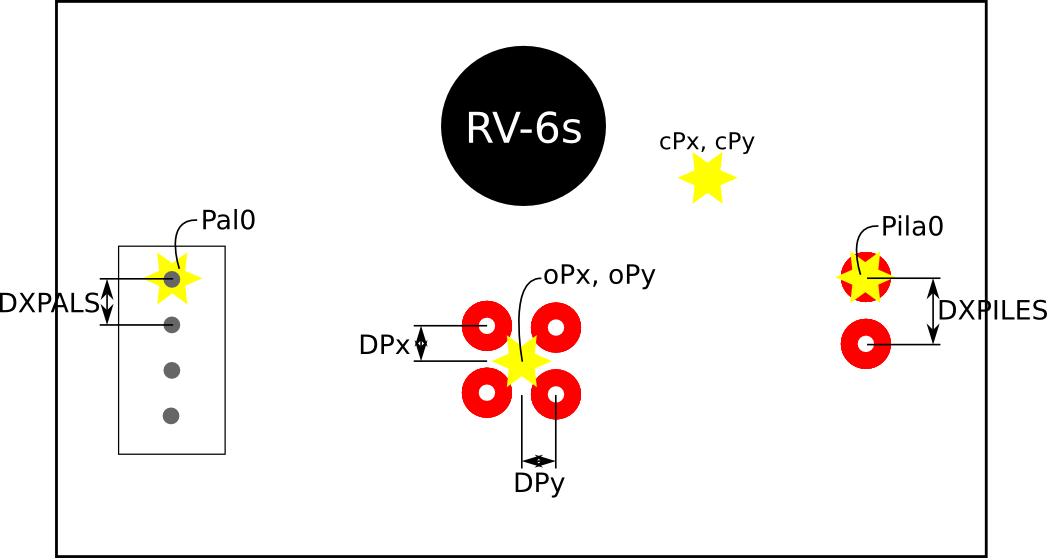
\includegraphics[width=0.8\textwidth]{escenari.png}
 % ordreRotacions.png: 1286x768 pixel, 150dpi, 21.77x13.00 cm, bb=0 0 617 369
\end{center}
  \caption{Escenari del robot}
\end{figure}

La figura es veu complementada amb el llistat de punts emprats a la pràctica.

\begin{minted}[frame=lines, fontsize=\small]{text}
DEF POS Paralisi = (337.16, -14.95, 270.30,-179.98, -0.36,-177.39)(7,0)
DEF POS Pal0     = (308.00,-550.00, 280.00, 171.00,-57.00, -79.00)(7,0)
DEF POS Pila0    = (340.18, 481.51, 280.00,-179.98, -0.36, -90.00)(7,0)
DEF POS Pale0    = (  0.00,   0.00, 280.00,-179.98, -0.36, -90.00)(7,0)
DEF POS PaleOut0 = (337.00,-450.00, 280.00, 171.00,-57.00, -79.00)(7,0)
\end{minted}

Com es detalla en l'apartat de \emph{calcul de punts} \ref{calcpts}
s'ha intentat minimitzar el nombre de punts capturats per tal
de calcular els demés en relació a aquests.

A continuació s'explica la utilitat de cada punt o posició.

\begin{description}
 \item [Paralisi] Guarda la posició del robot en repòs.
 \item [Pal0] Posició del primer pal (amb la pinça tombada).
 \item [Pila0] Posició de la primera pila (amb pinça perpendicular)
 \item [Pale0] Orientació del braç robot per posar peces del palé (amb la pinça
perpendicular).
 \item [PaleOut0] Orientació del braç robot per agafar les peces del palé
(amb la pinça tombada) 
\end{description}

A efectes pràctics a la imatge següent es veu el posicionat de les peces de una forma
humanament comprensible emprant les marques fetes per els alumnes sobre l'entorn i existents
a data de \today. 

\begin{figure}[H]
\begin{center}\label{fig:palmog}
 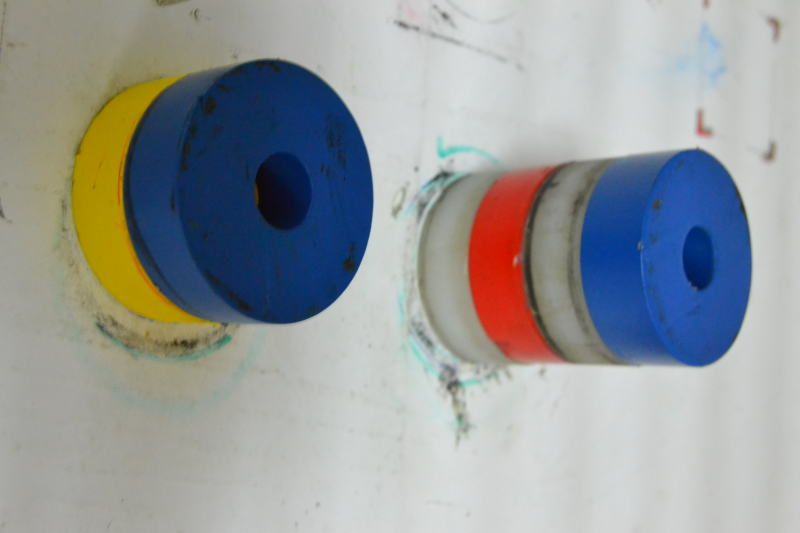
\includegraphics[width=0.8\textwidth,rotate=-90]{ubicacioPiles.jpg}
 % ordreRotacions.png: 1286x768 pixel, 150dpi, 21.77x13.00 cm, bb=0 0 617 369
\end{center}
  \caption{Posicionat de les piles a l'entorn}
\end{figure}

A la imatge es pot apreciar com la primera pila esta al centre fet amb
retolador negre i la segona seguint el cercle fet amb bolígraf \emph{Bic} blau.

Degut a l'esgotament de les bateries dels codificadors
angulars l'han hagut de re-calular les orientacions del braç, això provoca un
des-calibrat. El cas es que després del re-calibrat
del braç sempre quedava uns mi\lgem ímetres curt en l'eix \emph{Y}
per la introducció de les peces de tipus 4. Donat que l'eix \emph{Y}
es suposadament constant als quatre pals s'ha optat per moure la base en lloc d'ofuscar
el codi amb un cas especial. Concretament s'ha de rotar el suport dels
pals sobre el Pal0 en sentit anti-horari quedant el peu del costat del pal 3
com indica la figura \ref{palmog}. 

\begin{figure}[H]
\begin{center}\label{fig:palmog}
 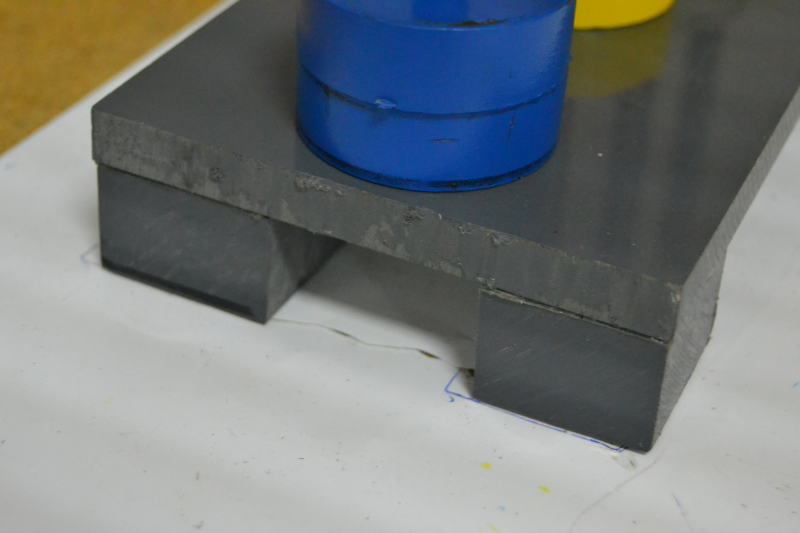
\includegraphics[width=0.8\textwidth]{palsMoguts.jpg}
 % ordreRotacions.png: 1286x768 pixel, 150dpi, 21.77x13.00 cm, bb=0 0 617 369
\end{center}
  \caption{Pals moguts, correcció després de l'esgotament de les bateries}
\end{figure}

Aquest fet es deu molt possiblement a lleugeres modificacions de l'orientació de la pinça
que s'han hagut de re-calcular, però que no s'ha ajustat més per l'inversió de temps
que suposa i que ja va fer-se al seu moment, així doncs seria feina duplicada sense sentit.

\section{Moviment del robot}
En aquest punt descrivim el moviment del braç robot i el perquè de l'ordre o
orientacions del mateix.

Totes les aproximacions a les peces es fan des de dalt. El braç robot es
posiciona a \emph{XY} sobre la peça en qüestió i després efectua un descens en \emph{Z}. Un
cop agafada efectua el moviment invers, ascens a Z i després el desplaçament
corresponent al pla \emph{XY} on es consideren segurs els moviments. Aquest pla de
seguretat en la pràctica ve donat per la variable \texttt{ZS} fixada per
defecte a 280.0.

En primer lloc el robot agafa les peces del les piles inicials.
Aquestes són co\lgem ocades a la zona de paletització. Ambdues
accions és duen a terme amb la pinça perpendicular al pla \emph{XY},
ja que es la posició més segura i còmode de programar per l'agafada
de peces.

Cal remarcar que la pinça esta mirant cap al vidre protector i la paret,
de tal manera que l'operador veu el metall. Aquest fet es deu a que
si no s'agafés bé la peça i aquesta sortís disparada ho faria en
direcció a la paret o el vidre protector, no cap a l'operari.

Un cop acabat el muntatge del palé és desmunta amb la pinça tombada,
s'agafen les peces començant per les que es
troben més a l'esquerra del braç robot, per co\lgem ocarles als pals.

El fet de tombar la pinça és per incrementar l'abast del braç robot. Amb la
pinça perpendicular al pla \emph{XY}, com s'havia efectuat el muntatge del palé, no
és possible arribar als pals 3 i 4. Com que s'ha decidit tombar la pinça
cap a l'esquerra\footnote{Els pals estan a la dreta del robot, per tant convé
tombar la pinça a la esquerra per simplificar els moviments i evitar haver
de fer un gir del braç}, des de el punt de vista del robot, s'han de recollir
les peces d'esquerra a dreta per tal de evitar que el braç co\lgem isioni
(fig. \ref{figcolisio}) amb algun dels munts del palé encara existents.

\begin{figure}[H]
\begin{center}
 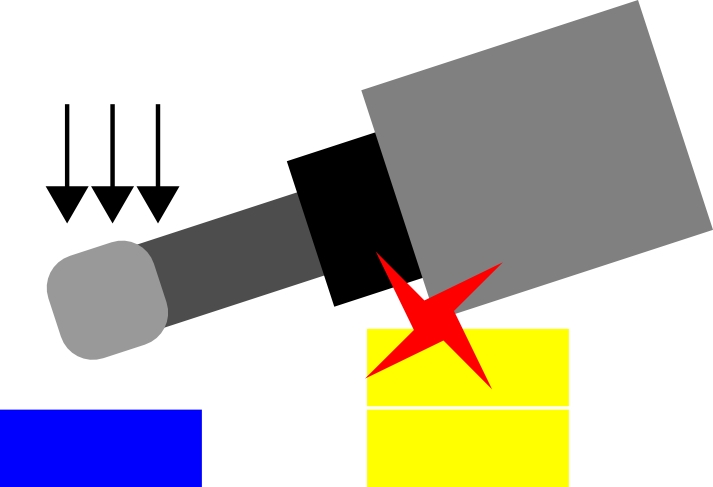
\includegraphics[width=0.6\textwidth]{colisio.png}
\end{center}
  \caption{Colisió amb el munt de peces grogues intentant agafar l'última peça blava}
\end{figure}\label{figcolisio}

Així doncs a la figura\ref{figrecpec}
veim quin seria l'ordre de recollida depenent dels diferents angles per tal
d'evitar les possibles co\lgem isions.

\begin{figure}[H]
\begin{center}\label{figrecpec}
 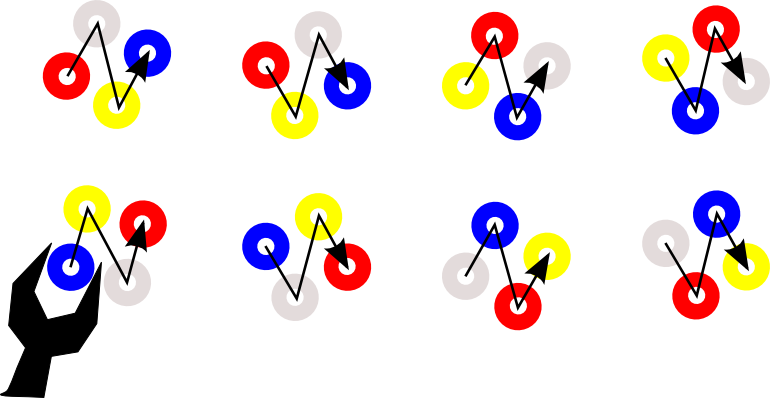
\includegraphics[width=0.8\textwidth]{ordreRotacions.png}
 % ordreRotacions.png: 1286x768 pixel, 150dpi, 21.77x13.00 cm, bb=0 0 617 369
\end{center}
  \caption{Ordre de recollida de les peces segons l'angle $\alpha$}
\end{figure}

Així doncs l'ordre de des-paletització depèn de l'angle i no del tipus de peça.
Com és pot veure a la figura existeixen 8 possibles casos que es veuen
reflectits en l'explicació del codi font corresponent, secció \ref{casosrot}.
  \newpage
  \section{Càlculs}
L'apartat de calculs inclou, per una banda, els requerits per l'encunicat a l'haver de transformar
el punt P del sistema de coordenades de la camera al del braç robot. En aquest punt es mostra
el procés de obtenció de les equacions per fer tal tranformació i en l'apartat de codi
es veu la seva implementació en el programa.

Per altra banda es mostra el calcul dels punts emprats de la situació dels objectes en l'entorn
a partir dels seus homolegs. Com s'ha mencionat la posició dels pals es relativa a un punt,
concretament tots els pals on es deixen les peces venen en funció de la posició del primer.
De la mateixa manera la posició de cada pila on inicialment es recullen les peces
ve en funció de la posició de la primera pila, el nombre de piles i la distància entre elles.
Finalment també es descriu el calcul de punts en Z on s'agafen les peces en funció del pla
de terra, l'altura de les peces i la quantitat de les mateixes.

\subsection{Transformació de sistemes de coordenades}
Amb l'enunciat tenim la posició de la càmera \{C\} respecte el robot \{R\} i
la posició del punt P, que es el centre de sistema de coordenades del palé \{P\},
respecte la càmera. El que volem es posar el punt P en el sistemes de coordenades del robot.

Així doncs definim:

\begin{description}
\item[$^RT_C$] La matriu de transformació de un punt del robot a la camera
\item[$^CT_P$] La matriu de transformació de un punt de la camera al palé
\item[$^PP$] Punt en el sistema de coordenades del palé
\item[$^RP$] Punt en el sistema de coordenades del robot
\end{description}

Combinant aquestes matrius obtenim que:

$$ ^RT_C \times \,^CT_P \times \,^PP = \,^RP $$

Per tant hem de cercar $^RT_P$:

$$ ^RT_P = \,^RT_C \times \,^CT_P $$

$$ ^RT_P = 
\left( \begin{array}{ccc|c}
0 & 1 &  0 & cPx\\
1 & 0 &  0 & cPy\\
0 & 0 & -1 &   0\\
\hline
0 & 0 &  0 & 1
\end{array} \right) \times
\left( \begin{array}{ccc|c}
cos \phi & -sin \phi &  0 & oPx\\
sin \phi &  cos \phi &  0 & oPy\\
0        &         0 &  1 &   0\\
\hline
0 & 0 &  0 & 1
\end{array} \right) $$

$$ ^RT_P = 
\left( \begin{array}{ccc|c}
sin \phi &  cos \phi &  0 & oPy + cPx\\
cos \phi & -sin \phi &  0 & oPx + cPy\\
0        &         0 & -1 &   0\\
\hline
0 & 0 &  0 & 1
\end{array} \right)$$

Així doncs per passar d'un punt del sistema de coordenades $^PP$ a $^RP$ ho feim així:

$$^RT \times \,^PP = \,^RP$$

En el cas generic agafam $^PP = 
\left( \begin{array}{c}
x \\
y \\
z \\
\hline
1
\end{array} \right)$

$$
\left( \begin{array}{ccc|c}
sin \phi &  cos \phi &  0 & oPy + cPx\\
cos \phi & -sin \phi &  0 & oPx + cPy\\
0        &         0 & -1 &   0\\
\hline
0 & 0 &  0 & 1
\end{array} \right)
\times
\left( \begin{array}{c}
x \\
y \\
z \\
\hline
1
\end{array} \right)
=
\left( \begin{array}{c}
x\times sin \phi + y \times cos \phi + cPy + cPx \\
x\times cos \phi - y \times sin \phi + oPx + cPy \\
-z \\
\hline
1
\end{array} \right)
$$

De on extreim les següents equacions que seran implementades dins del
nostre programa. TODO LABEL

$$^RP_X = x\times sin \phi + y \times cos \phi + cPy + cPx$$
$$^RP_Y = x\times cos \phi - y \times sin \phi + oPx + cPy$$
$$^RP_Z = -z$$

\subsection{Calcul de piles, pals (X,Y) i altura de peces (Z)}
A banda de la transformació de punts entre sistemes de coordenades hi ha altres punts a calcular.
El primer son les piles d'on s'agafen les peces. Dins del llistat de punts tenim el punt de la primera
pila, les següents es troben situades a un desplaçament en Y. Així doncs en el nostre escenari
senzillametn s'ha de incrementar en Y el valor de la distancia entre piles. Succeeix exactament
el mateix amb els pals on es deixen les peces.

Els detalls de implementació i valors de les constants de separació es poden veure en l'apartat
especifíc TODO LABEL on s'explica el codi font. Cal remarcar que al codi tambe figura un
desplaçament en X, per si es volguessin posar les piles o pals fent una diagonal, però la \emph{macro}
esta inicialitzada a 0.





  \newpage
  \section{Estructura del programa}
El programa es divideix en cinc seccions.

\begin{description}
\item [Capçalera de l'enunciat] Interfície de \emph{macros} requerida
per l'enunciat on hi ha paràmetres com l'angle $\alpha$.

\item [Macros pròpies] Reassingació de valors per les funcionalitats extra que
s'han implementat com ara emprar piles amb nombre de peces diferets, si es vol
fer una execució amb l'enunciat original sols fa falta assignar els valors de
les variables de la secció anterior.

\item [Declaracions pròpies] Aquí es declaren les variables globals pròpies
del programa, en principi sols les ha de tocar el programador.

\item [Rutines] Codi de les rutines on es desenvolupa tota la pràctica.

\item [Main] Simple crida ordenada a les rutines per desencadenar l'execució.
\end{description}

\subsection{Macros, paràmetres}
Les \emph{macros}\footnote{Cal mencionar que aquests valors no són realment
\emph{macros} sinó variables, una \emph{macro} es resol en temps de
pre-processador no en temps de compilació o execució, el fet de que el
llenguatge no disposi de \emph{macros} porta alguns problemes mencionats
a l'apartat de incidents\ref{incmaros}.} de la \emph{capçalera de l'enunciat} 
ja estan explicades al propi enunciat, aquí s'expliquen les altres
\emph{macros} introduïdes per les funcionalitats pròpies, corresponents a
l'apartat de \emph{Macros pròpies}.

\begin{description}\label{macprop}
\item [PINCA] Valor de la pinça emprada, en el nostre cas el robot només en té
una i és la 1.

\item [DPALE] Retard (\emph{D}elay) de 4 segons requerit a l'enunciat un cop
s'ha muntat el palé.

\item [D\#PINCA\%] Retards aplicats després de \emph{O\#}brir o
\emph{T\#}ancar la pinça en funció de si es \emph{I\%}nicial o \emph{F\%}inal,
abans o després d'agafar la peça.

\item [VLENT] \emph{V}elocitat a la qual es duen a terme les aproximacions
delicades, com l'agafada de peces.

\item [VNORMAL] \emph{V}elocitat a la que es desplaça normalment el braç en els
trajectes segurs.

\item [ZS] Pla \emph{Z} on es consideren segurs els moviments del braç robot i on
es duen a terme els desplaçaments llargs.

\item [ZTPT] Pla de \emph{T}erra ($Z = 0$) amb la \emph{P}inça \emph{T}ombada
(angle inferor a 45 amb el pla \emph{XY})

\item [ZTPR] Pla de terra amb la pinça perpendicular al pla \emph{XY}  
                                                                                                         
\item [TP] \emph{T}ipus de \emph{P}eça diferents que tenim, es igual el
número de munts del palé i de pals de destí.

\item [PILES] Número de piles d'on es fa la recollida inicial de peces.

\item [PALS] Número de pals de destí on es deixen les peces.

\item [DT] Retard per l'obertura i tancament de la pinça.

\item [HDISC] Altura de les peces (discs)

\item [D\#PILES] Distància en \emph{X} i \emph{Y} entre les piles

\item [D\#PALS] Distància en \emph{X} i \emph{Y} entre els pals

\item [DZPAL] Distància \emph{Z} a baixar per introduir la peça dins el pal.

\item [RELPALE(T,E)] Distància relativa de la peça tipus \emph{T} al punt
\emph{P}, en funció de l'eix \emph{E} (1 per \emph{X}, 2 per \emph{Y})
\end{description}

\subsection{Estructura del codi}
En el codi s'ha fet una funció per cada acció i alguna d'auxiliar transversal.
La intenció es dedicar tota la feina a les rutines i que la lectura del
programa es pugui llegir de manera natural en els nivells més alts entrant en
detalls a mesura que es va aprofundint en les funcions.

\begin{center}
\begin{tabular}{|l|l|l|l|}
\hline
\multicolumn{2}{|c|}{Munta palé} & \multicolumn{2}{|c|}{Desmunta palé}\\
\hline
Agafa pila & Posa palé & Agafa Palé & Posa pal\\
\hline
\multicolumn{4}{|c|}{Obre/tanca pinça}\\
\hline
\end{tabular}
\end{center}


Cal fer especial menció a dos vectors de control de l'estat del programa,
aquests són \texttt{npcspila} i \texttt{alloc}.

\texttt{npcspila(p)} conté el nombre de peces que resten a la pila inicial d'
on s'agafen les peces.

\texttt{alloc(m)} indica quantes peces ja estan a lloc, situades al munt
\texttt{p} del palé, recordem que cada munt correspon a un tipus de peça.

Ambdues variables serveixen per controlar l'altura en \emph{Z} d'on agafar les
peces, i per sabre quan ja no en queden més.

Amb aquest principi ens queda un cos principal tan lleuger com aquest.
\begin{minted}[frame=lines, fontsize=\small]{vbnet}
970 gosub *INIT
980 gosub *CALCPTS
990 gosub *MNTPALE
1000 dly DPALE
1010 gosub *DESPALE
1020 gosub *ACABA
1030 end
\end{minted}

\subsubsection{Auxiliars}
\paragraph{Canvi sistemes de coordenades}\label{cam2rob}
En la funció \texttt{CAM2ROB} es troba implementat el canvi de sistemes
de coordenades del la càmera al robot.
Com a interfície llegeix els punts \texttt{ppx} i \texttt{ppy} que són els que es desitgen
transformar, així com les \emph{macros} del programa \texttt{oPx}, \texttt{oPy},
\texttt{cPx}, \texttt{cPy} i l'\texttt{angle}. Deixa els valors de
\texttt{ppx} i \texttt{ppy} en funció del sistema de coordenades del braç
robot en les variables \texttt{prx} i \texttt{pry}.

\begin{minted}[frame=lines, fontsize=\small]{vbnet}
2020 *CAM2ROB
2030 	angleR =(angle*M_PI) / 180.0
2040    prx = ppx*sin(angleR) + ppy*cos(angleR) + oPy + cPx
2050    pry = ppx*cos(angleR) - ppy*sin(angleR) + oPx + cPy
2060    return
\end{minted}

\paragraph{Obertura-Tancament de pinça}
Per tal de facilitar la llegibilitat del codi i no afegir constantment
els retards per la obertura i tancament de pinça s'han definit les funcions
\texttt{OPINCA} i \texttt{TPINCA} que encapsulen aquest comportament.

\begin{minted}[frame=lines, fontsize=\small]{vbnet}
2080 *OPINCA
2090    dly DOPINCAI
2100    hopen PINCA
2110    dly DOPINCAF
2120    return
\end{minted}
\begin{minted}[frame=lines, fontsize=\small]{vbnet}
2130 *TPINCA
2140    dly DTPINCAI
2150    hclose PINCA
2160    dly DTPINCAF
2170    return
\end{minted}

\subsubsection{Inicialitzacions}
En aquesta rutina es duu a terme l'operació de \emph{homing} i demés
inicialitzacions físiques del braç robot com l'obertura de la pinça
o de les variables que controlen l'entorn del robot, com el 
comptador de peces que s'han posat a cada palé.

\begin{minted}[frame=lines, fontsize=\small]{vbnet}
1050 *INIT
1060    servo ON
1070    ovrd VNORMAL
1080    mov Paralisi
1090    gosub *OPINCA
1100    for i = 1 to TP
1110        alloc(i) = 0
1120    next
1130    return
\end{minted}

\subsubsection{Càlcul de punts}\label{codcalcpts}
Com ja s'ha comentat en la pràctica s'ha fet el màxim esforç per posar tots els
punts en funció d'uns pocs, per això en la funció de càlcul de punts s'omplen
els vectors que contenen els punts homòlegs calculats a partir de les
\emph{macros} que descriuen l'entorn físic. En aquest punt també es calcula
l'ordre de recollida de les peces en funció de l'angle\ref{figrecpec}. Per limitacions del
llenguatge comentades a l'apartat de incidents TODO LABEL el codi no has
sortir gaire elegant.

Un cop acabada la funció càlcul de punts tots els vectors de punts estan apunt
per ser recorreguts per part del braç robot en els eixos (X,Y), el Z és
calculat en temps d'execució ja que depèn de quina peça s'estigui tractant,
ja que son apilades a l'eix Z.
Aquests vectors emprats de interfície són:

\begin{description}
 \item [\texttt{Pila}] Cada component indica la posició (X,Y) de cada una de
les piles d'on s'agafen
inicialment les peces, en l'execució per defecte seran dues.
 \item [\texttt{Pale}] Cada component correspon a la posició on anirà
co\lgem ocat cada tipus de peça al palé.
 \item [\texttt{PalI}] Posició inicial on es co\lgem coca el braç per iniciar
el descens sobre el pal.
 \item [\texttt{PalF}] Punt final de descens del braç, on es considera que la
peça ja hi ha entrat i pot ser amollada.
\end{description}

\label{casosrot}
\begin{minted}[frame=lines, fontsize=\small]{vbnet}
1140 *CALCPTS
1150    for pil = 1 to PILES
1160        Pila(pil) = Pila0
1170        Pila(pil).x = Pila(1).x + DXPILES * (pil - 1)
1180        Pila(pil).y = Pila(1).y + DYPILES * (pil - 1) 'es 0
1190    next
    
1210    for tipus = 1 to TP
1220        ppx = RELPALE(tipus, 1) 'paramentres de entrada de CAM2ROB
1230        ppy = RELPALE(tipus, 2)
1240        gosub *CAM2ROB           'prx i pry son parametres de sortida
1250        Pale(tipus) = Pale0    'Escriu altres components i orientacions
1260        Pale(tipus).x = prx
1270        Pale(tipus).y = pry
1280        PaleOut(tipus) = PaleOut0
1290        PaleOut(tipus).x = prx '- 7.0
1300        PaleOut(tipus).y = pry - 15.0
1310    next
 
1330    for pal = 1 to PALS
1340        PalI(pal) = Pal0
1350        PalI(pal).x = PalI(pal).x + DXPALS * (pal - 1)
1360        PalI(pal).y = PalI(pal).y + DYPALS * (pal - 1)
1370        PalF(pal) = PalI(pal)
1380        PalF(pal).z = PalF(pal).z - DZPAL
1390    next
1400 	
1410    angle = angle mod 360
1420    if ((0.0 < angle) and (angle < 45.0)) then
1430        ordre(1) = 3
1440        ordre(2) = 2
1450        ordre(3) = 4
1460        ordre(4) = 1
1470        return
1480     endif
1490    if ((45.0 < angle) and (angle < 90.0)) then 
1500        ordre(1) = 3
1510        ordre(2) = 4
1520        ordre(3) = 2
1530        ordre(4) = 1
1540        return
1550    endif
1560    if ((90.0 < angle) and (angle < 135.0)) then
1570        ordre(1) = 4
1580        ordre(2) = 3
1590        ordre(3) = 1
1600        ordre(4) = 2
1610        return
1620    endif
1630    if ((135.0 <= angle) and (angle < 180.0)) then
1640        ordre(1) = 4
1650        ordre(2) = 1
1660        ordre(3) = 3
1670        ordre(4) = 2
1680        return
1690    endif
1700    if ((180.0 <= angle) and (angle < 225.0)) then 
1710        ordre(1) = 1
1720        ordre(2) = 4
1730        ordre(3) = 2
1740        ordre(4) = 3
1750        return
1760    endif
1770    if ((225.0 <= angle) and (angle < 270.0)) then
1780        ordre(1) = 1
1790        ordre(2) = 2
1800        ordre(3) = 4
1810        ordre(4) = 3
1820        return
1830    endif
1840    if ((270.0 <= angle) and (angle < 315.0)) then 
1850        ordre(1) = 2
1860        ordre(2) = 1
1870        ordre(3) = 4
1880        ordre(4) = 3
1890        return
1900    endif
1910    ' 315.0 > angle < 360.0
1920    ordre(1) = 2
1930    ordre(2) = 3
1940    ordre(3) = 1
1950    ordre(4) = 4
1960    return
\end{minted}

\subsubsection{Munta palé}
Tal i com indica el títol en aquesta funció es munta el palé, aquesta tasca
consisteix en iterar per cada una de les peces existents en cada una de les
piles per agafar-les i depositar-les al lloc corresponent del palé.

\begin{minted}[frame=lines, fontsize=\small]{vbnet}
2180 *MNTPALE
2190    peca = 1
2200    for pil = 1 to PILES 
2210        for pecapila = 1 to npcspila(pil)
2220            gosub *AGAFPILA
2230            gosub *POSAPALE
2240            peca = peca + 1
2250        next
2260    next
2270    return
\end{minted}

\paragraph{Agafa de la pila}
\begin{minted}[frame=lines, fontsize=\small]{vbnet}
2380 *AGAFPILA
2390    mov Pila(pil)
2400    Prvsnl = Pila(pil)
2410    Prvsnl.z = Prvsnl.z - ZTPR + (npcspila!(pil) - pecapila) * HDISC
2420    ovrd VLENT
2430    mvs Prvsnl
2440    gosub *TPINCA
2450    mvs Pila(pil)
2460    ovrd VNORMAL
2470    return
\end{minted}

\paragraph{Posa al Palé}
\begin{minted}[frame=lines, fontsize=\small]{vbnet}
2480 *POSAPALE
2490    mov Pale(tipusP(peca))
2500    Prvsnl = Pale(tipusP(peca))
2510    Prvsnl.z = Prvsnl.z - ZTPR + alloc(tipusP(peca)) * HDISC
2520    ovrd VLENT
2530    mvs Prvsnl
2540    gosub *OPINCA
2550    mvs Pale(tipusP(peca))
2560    ovrd VNORMAL
2570    alloc(tipusP(peca)) = alloc(tipusP(peca)) + 1
2580    return
\end{minted}

\subsubsection{Desmunta palé}
En aquest punt del programa el braç va munt a munt del palé agafant les peces
i deixant-les als pals, no passa al següent munt mentre a l'actual quedin peces.
L'ordre d'agafada dels munts ha estat calculat en \emph{càlcul de punts} com ja s'ha
esmentat\ref{codcalcpts}.

\begin{minted}[frame=lines, fontsize=\small]{vbnet}
2290 *DESPALE
2300    for tipus = 1 to TP
2310        munt = ordre(tipus)
2320        while alloc(munt) > 0
2330            gosub *AGAFPALE
2340            gosub *POSADEST
2350        wend
2360    next
2370    return
\end{minted}

\paragraph{Agafa del palé}
\begin{minted}[frame=lines, fontsize=\small]{vbnet}
2590 *AGAFPALE
2600    mov PaleOut(munt)
2610    Prvsnl = PaleOut(munt)
2620    Prvsnl.z = Prvsnl.z - ZTPT + (alloc(munt) - 1) * HDISC
2630    ovrd VLENT
2640    mvs Prvsnl
2650    gosub *TPINCA
2660    mvs PaleOut(munt)
2670    ovrd VNORMAL
2680    alloc(munt) = alloc(munt) - 1
2690    return
\end{minted}

\paragraph{Posa pal}
\begin{minted}[frame=lines, fontsize=\small]{vbnet}
2700 *POSADEST
2710    mov PalI(munt)
2720    ovrd VLENT
2730    mvs PalF(munt)
2740    gosub *OPINCA
2750    mvs PalI(munt)
2760    ovrd VNORMAL
2770    return
\end{minted}

\subsubsection{Acaba}
De manera similar a l'inicialitza, acaba s'encarrega del posicionament
físic del robot en una posició de repòs i la desconnexió dels servomotors.

\begin{minted}[frame=lines, fontsize=\small]{vbnet}
1970 *ACABA
1980    mov Paralisi
1990    hopen PINCA
2000    servo OFF
2010    return
\end{minted}


  \newpage
  \section{Joc de proves}

Per tal de provar la pràctica s'han realitzat una sèrie de jocs de proves
descrits a continuació.

Els primers es realitzen amb l'enunciat per defecte, sols dos munts i
quatre peces, una de cada tipus. A continuació es duen a terme rotacions
del palé.

Cada una de les rotacions es fa per comprovar que el braç agafi les
peces amb l'ordre que toca sense co\lgem isonar amb els demés munts.
Així doncs es realitzen 8 execucions corresponents als 8 casos
\ref{figrecpec} de recollida que s'han esmentat a l'apartat
d'explicació de l'enunciat.

A continuació es realitza la prova de posar les 4 paces del mateix tipus,
aquest test serveix per comprovar si funciona correctament el desplaçament
en \emph{Z}. Per altra banda amb aquest test es comprova que passa
quan no existeix algun tipus de peça en la seqüència.

Finalment es prova l'execuió amb piles de diferent dimensió (4 i 2)
amb peces repetides del mateix color.

Cal esmentar que tots els tests foren passats abans de l'escotament
de les bateries que guardaven els valors dels codificadors angulars
òptics. Després del reestabliment del robot sols s'han fet proves
amb les piles de diferent tamany amb $\alpha = 133$ i $\alpha = 240$.
  \newpage
  \section{Incidents, problemàtica al desenvolupament i valoració}\label{incidents}

Durant el desenvolupament com es habitual hom es troba amb problemes a resoldre,
alguns d'ells fruit de l'aprenentatge però d'altres deguts a limitacions
de l'entorn ja sigui físic com virtual.

\subsection{Problemàtica física}

El primer problema a afrontar era fer arribar les peces als pas 3 i 4. 
S'entén que aquest fet es intencionat per complicar una mica
més la pràctica. En el nostre cas això ha estat resolt tombant la pinça com ja s'ha exposat en
les seccions anteriors. El fet de tombar la pinça porta una sèrie complicacions 
addicionals. L'una és que el sistema de coordenades de la pinça no està
ubicat perfectament a la zona de contacte on s'agafen les peces, això fa que
s'hagi de fer una petita correcció en \emph{XY} respecte
a la posició quan està perpendicular. Aquesta correcció és veu al codi com una
resta de 17.0 a \emph{Y}, no definit com a \emph{macro} per resignació.

La so\lgem ució no es gaire elegant però si efectiva, tal vegada si el 
treball a realitzar fos més complexe consideraríem intentar moure el sistema
de coordenades al punt correcte, ja sigui amb la funció \texttt{tool}
com fent un càlcul propi a mà i tenint una funció similar a la \texttt{CAM2ROB}
(secció \ref{cam2rob}).

En l'entorn físic també ens hem trobat amb el problema que les peces
tenen restes de cola i vegades s'aferren entre elles movent dues peces a la
vegada, cosa que desbarata totalment l'execució i requereix un reseteig manual
de l'entorn.

S'entén que tots aquests problemes físics són fruit de viure en un món
material amb certes complicacions que, al cap i a la fi, fan la vida un poc més
interessant. Per altra banda si entram en l'apartat de problemes o incidents
en el programari ens trobam amb coses menys justificables.

\subsection{Problemàtica virtual}

El llenguatge de programació del robot es un autèntic desastre, incòmode i
poc pràctic. A classe s'ha comentat que una de les problemàtiques de la robòtica 
industrial és el temps que és té el robot aturat per programar-lo i 
d'aquí que s'inverteixi molt de temps en simuladors, que no poden, entre d'altres, simular
els problemes físics esmentats anteriorment. Així doncs seria molt més
eficaç tenir millors llenguatges que no indueixin a l'error i facilitin
un desenvolupament més ràpid que no pas dedicar-se a simuladors.

Concretament al llenguatge li sobren coses com el numerat de línia,
sobretot que l'entorn no ho faci de manera completament automàtica.
Requerir numerat només fa que s'hagi de pitjar el botó de re-enumeració
cada cop i esperar que es faci el procés, que incomprensiblement tarda
uns 2 o 3 segons.

Al llenguatge també són necessaris més elements, el primordial són
variables locals i crides de funcions amb un fàcil pas de paràmetres,
les variables globals i el \texttt{gosub} indueixen freqüentment a l'error.

Falta de \emph{macros}, en tot programa, i més els que tracten entorns físics,
són necessaris números màgics, aquests poden ser resolts amb una variable
però si són necessaris per la declaració d'un vector tenim un problema,
i més si el llenguatge no permet que aquests siguin dinàmics. És
trist haver de posar números màgics per tot amb un comentari el costat
on aparegui algun identificador per poder-los localitzar al llarg del codi
quan s'ha de realitzar algun canvi.

Tampoc estaria de més el suport de la funció de \texttt{case} amb \texttt{floats} 
o com a mínim l'entorn podria aixecar un advertiment en ser usat, dient que no funciona.

Finalment comentar que el sistema de mostrat d'errors pobre a més de sovint
pràcticament inexistent.

\subsection{Valoració}
Aquests comentaries venen perquè l'algorisme i modelat de la pràctica s'elaboraren
en unes hores. El gruix de temps invertit ha estat ajustant paràmetres del robot i barallant-se
amb el llenguatge i entorn. Així i tot ha estat d'agrair el fet de poder estar amb contact amb un braç
real. Cal dir que tot i així la pràctica ha estat amena i entretinguda, però en aquests
temps convé més ser critic per millorar encara més el que és té, intentant que cada cop la Universitat
sigui un millor lloc per el creixement de l'estudiant.

 \let\thefootnote\relax\footnotetext{
 Aquest document està baix llicència \href{http://creativecommons.org/licenses/by-sa/3.0/}{Creative Commons Atributive Share-Alike 3.0}
 per tant es pot compartir, modificar i distribuir, però citant els autors originals i sense modificar la llicència.
 De la mateixa manera el codi font està baix llicència GNU GPL v3 per part dels dos autors.\bigskip}
\let\thefootnote\relax\footnotetext{El document en versió digital i el codi font el trobareu a \\ \url{https://github.com/bmiro/raiden}\bigskip}
\let\thefootnote\relax\footnotetext{Aquest document i tota la part de la practica que s'ha pogut ha estat desenvolupat emprant programari lliure:}
\let\thefootnote\relax\footnotetext{\href{http://www.tug.org/applications/pdftex/}{\LaTeX} i \href{http://www.tug.org/applications/pdftex/}{Kile} per el text,
\href{http://www.inkscape.org/}{Inkscape} pels diagrames,
\href{http://kate-editor.org/}{Kate} i \href{http://vim.org/}{Vim} per l'edició del codi font.
\href{http://git-scm.com/}{Git} com a sistema de control de versions.
}

\let\thefootnote\relax\footnotetext{
\begin{center}
\begin{tabular}{cc}

\includegraphics[height=35pt,keepaspectratio=true]{diagrames/by-sa.png}
 & 
\includegraphics[height=35pt,keepaspectratio=true]{diagrames/gnu.png}
\end{tabular}
\end{center}
\begin{center}
\begin{tabular}{cccccc}
 
\includegraphics[height=35pt,keepaspectratio=true]{diagrames/latex.png}
 & 
\includegraphics[height=35pt,keepaspectratio=true]{diagrames/kile.png}
 & 
\includegraphics[height=35pt,keepaspectratio=true]{diagrames/inkscape.png}
 & 
\includegraphics[height=35pt,keepaspectratio=true]{diagrames/kde.png}
 & 
\includegraphics[height=35pt,keepaspectratio=true]{diagrames/vim.jpg}
 & 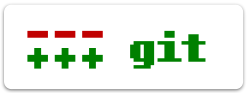
\includegraphics[height=35pt,keepaspectratio=true]{diagrames/git.png}
\end{tabular}
\end{center}
}
   \let\thefootnote\relax\footnotetext{
 Aquest document està baix llicència \href{http://creativecommons.org/licenses/by-sa/3.0/}{Creative Commons Atributive Share-Alike 3.0}
 per tant es pot compartir, modificar i distribuir, però citant els autors originals i sense modificar la llicència.
 De la mateixa manera el codi font està baix llicència GNU GPL v3 per part dels dos autors.\bigskip}
\let\thefootnote\relax\footnotetext{El document en versió digital i el codi font el trobareu a \\ \url{https://github.com/bmiro/raiden}\bigskip}
\let\thefootnote\relax\footnotetext{Aquest document i tota la part de la practica que s'ha pogut ha estat desenvolupat emprant programari lliure:}
\let\thefootnote\relax\footnotetext{\href{http://www.tug.org/applications/pdftex/}{\LaTeX} i \href{http://www.tug.org/applications/pdftex/}{Kile} per el text,
\href{http://www.inkscape.org/}{Inkscape} pels diagrames,
\href{http://kate-editor.org/}{Kate} i \href{http://vim.org/}{Vim} per l'edició del codi font.
\href{http://git-scm.com/}{Git} com a sistema de control de versions.
}

\let\thefootnote\relax\footnotetext{
\begin{center}
\begin{tabular}{cc}

\includegraphics[height=35pt,keepaspectratio=true]{diagrames/by-sa.png}
 & 
\includegraphics[height=35pt,keepaspectratio=true]{diagrames/gnu.png}
\end{tabular}
\end{center}
\begin{center}
\begin{tabular}{cccccc}
 
\includegraphics[height=35pt,keepaspectratio=true]{diagrames/latex.png}
 & 
\includegraphics[height=35pt,keepaspectratio=true]{diagrames/kile.png}
 & 
\includegraphics[height=35pt,keepaspectratio=true]{diagrames/inkscape.png}
 & 
\includegraphics[height=35pt,keepaspectratio=true]{diagrames/kde.png}
 & 
\includegraphics[height=35pt,keepaspectratio=true]{diagrames/vim.jpg}
 & 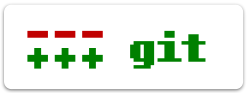
\includegraphics[height=35pt,keepaspectratio=true]{diagrames/git.png}
\end{tabular}
\end{center}
}


\end{document}
